\chapter{Unreal Engine}\label{chp:UnrealEngine}

The Unreal Engine is a 3D graphics video game engine, first created for the first person shooter Unreal in 1998\cite{UnrealWiki}. Originally written mostly by Tim Sweeney, the founder of Epic Games, it has since grown an incredible amount and become one of the most popular game engines on the market, only perhaps beaten by Unity\cite{}. It has also had many versions since its initial release, first with Unreal Engine 2 in 2002 and then with version 3 in 2006\cite{}. Up until recently Unreal Engine 4, released in 2014, was the latest version but April of 2022 saw the official release of Unreal Engine 5. All of the versions were written in C++ enabling great performance as well as portability, so that the engine is currently supported on a wide range of desktop, console, mobile and even virtual reality platforms\cite{}.\\

In its more than 25 year history the Unreal Engine has been used to create a vast number of incredibly popular and critically acclaimed games such as Fortnite, Hellblade and the Bioshock series, only to name a few. Even though the main use-case has remained video game development, the engine has seen wide adoption in many other industries as well. In film making it can be used to create virtual sets that can be rendered in real time on large LED screens and lighting systems while also tracking around actors and objects using the camera's movement. Epic Games worked with the Industrial Lights and Magic of division Lucasfilm to develop their StageCraft technology\cite{StageCraft}, first used in filming the television show The Mandalorian\cite{Mando}. Outside of these creative fields due to its wast functionalities and ease of use, it has been used to create virtual reality tools to explore building and car designs, as well pharmaceutical drug molecules\cite{unrealwiki}.\\

For the purposes of this project Unreal Engine 4.27 was used and this is the version that will be described unless specified otherwise. Although this technically isn't the latest version and the development of this project started around the same time as version 5 was officially released, there were multiple reason as to why this decision was made. First of all, pretty much any new software release tends to bring with it a number of bugs and quirks which need to be discovered and fixed first. This doesn't always have to be the case but a lot of developers will wait for the software become more ironed out before using it. That is if they even want to use UE5. There are many programs already written in earlier versions of it and not every one of those might truly require the new features UE5 brings with it so the update might not even occur. Also the initial research for the project, which also included learning how Unreal works and how to use it, was done months before the launch.\\ On the other hand Unreal Engine 4 is a very mature tool which has been used and improved for years now. There are also many sub-versions of it but the decision was made to use the latest one, 4.27.2, as it should be UE4 at its best and also due to the excellent compatibility between it and earlier version of UE4.

%%%%%%%%%%%%%%%%%%%%%%%%%%%%%%%%%%%%%%%%%%%%%%%%%%%%%%%%%%%%%%%%%%%%%%%%%%%%%%%%%%%%%%%%%%%%%%%
\section{Unreal Engine Basics}\label{sec:Grundlage1}
Developing a video game is quite a complicated process and requires various features in order to create a cohesive experience. As Unreal is primarily a game development engine it also has to support many of these functionalities. In total there are more than dozen editors for levels, materials, meshes,physics and user-interface, to just name a few, but for the purposes of this project only a few are of relevance. These are the level, material and blueprint editors.\\

The level editor is the primary editor where the levels are created and modified by placing, transforming and editing properties of objects. This is also the default screen Unreal shows when creating or opening a project and what that looks like is shown in figure \ref{fig:LevelEditor}. As can be seen in the figure, in the centre of the screen is the level itself. Above it is a toolbar for managing project settings, code, plug-ins and as well a play button which can be used to launch the game inside of the editor for testing purposes. On the bottom the content browser which display all of the assets which are part of the project can be found. This includes meshes, materials, code as well as project plug-ins. On the left is a toolbar for placing various built in objects and on the right all of the objects in the current world, as well as details about the currently selected object can be seen.\\
This is also generally the screen where a developer would import any external assets into the engine directly or through one of the engines importer tools.\\

\begin{figure}[htpb]
	\centering
	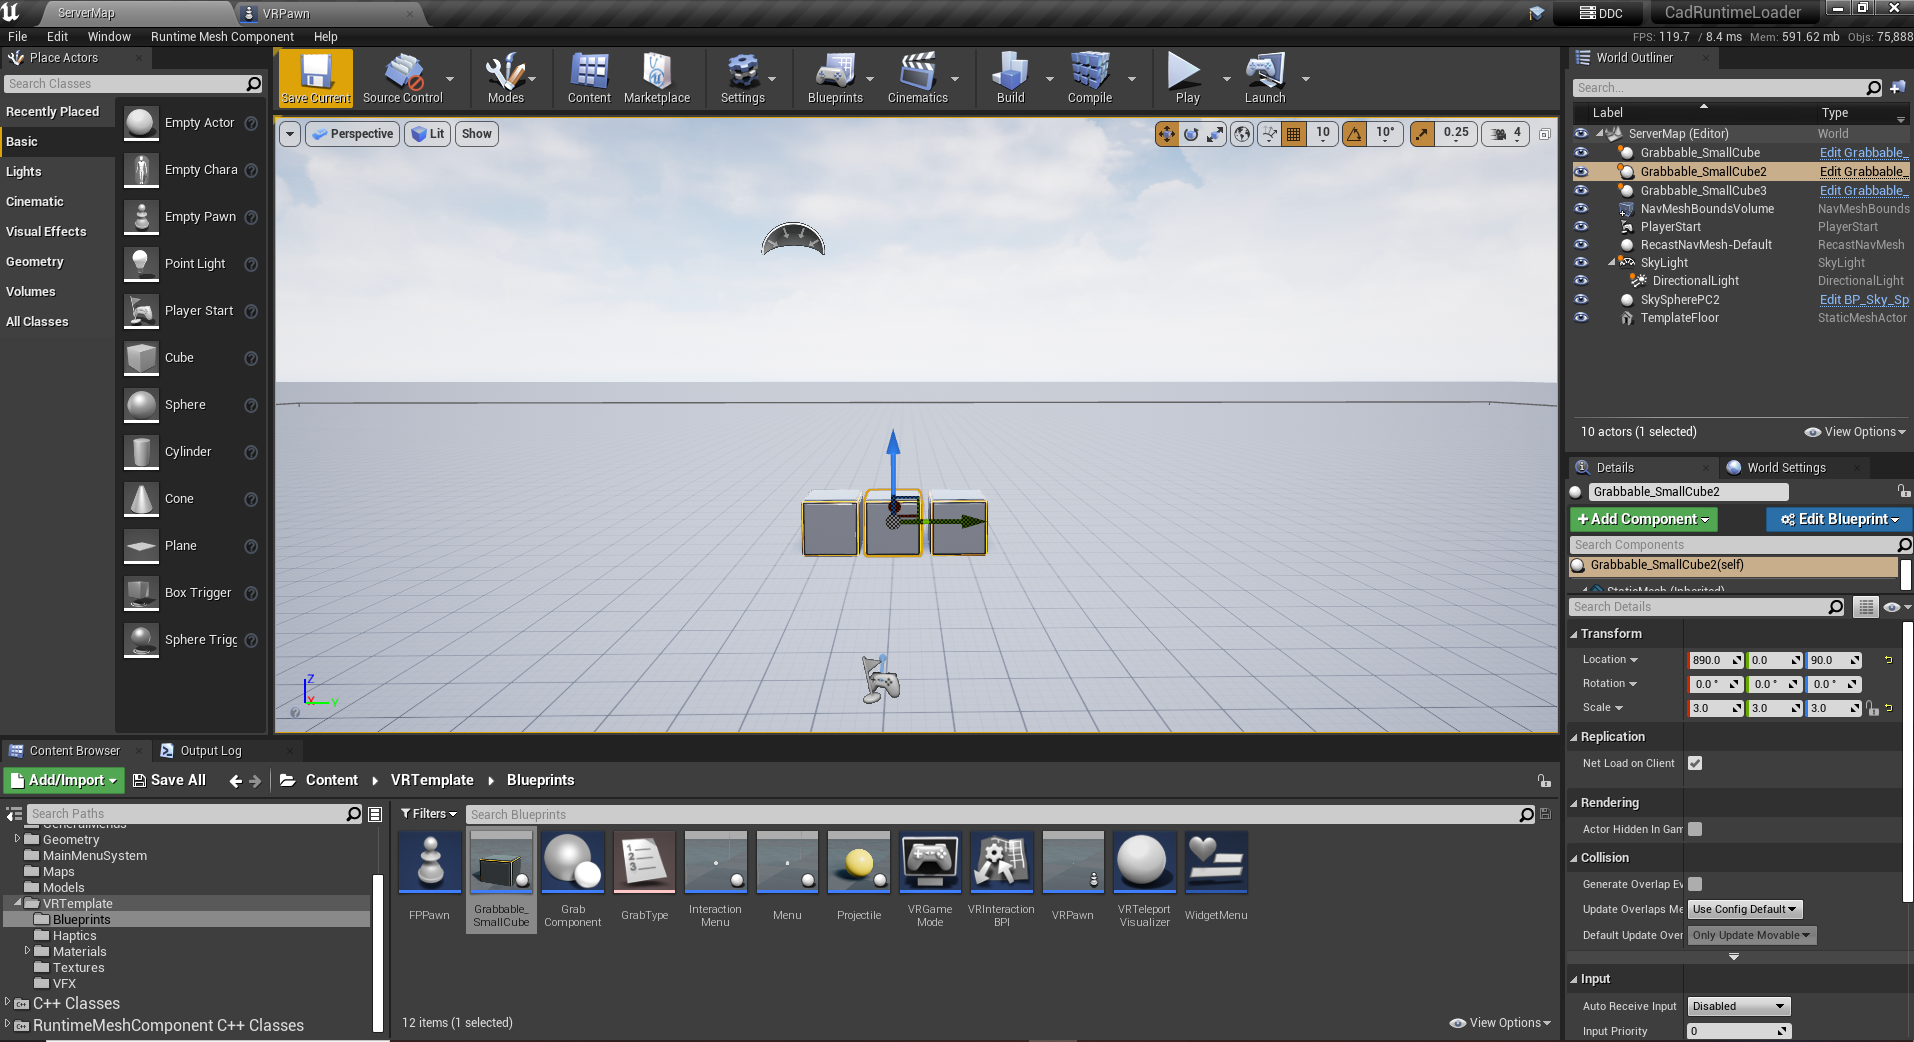
\includegraphics[width=0.9\textwidth]{fig/UnrealEngineLevelEditor.png}
	\caption[Unreal Engine Level Editor]{Example of what the Level Editor looks like for a project \protect}
	\label{fig:LevelEditor}
\end{figure}

\subsubsection{Actors and Components}
%Describ Actors and Components and world and local coordinates, detaching

In Unreal Engine all of the objects that can be placed inside of a level are called Actors. This includes everything from meshes to particle systems to even the players starting location. This is partially due to Unreal Engines object-oriented nature so having all objects inherit from one base class, in this case Actor, can be quite beneficial.

\subsubsection{Pawns and Player Controllers}
%what pawns are and what a player controller is, what they are used for and what their purposes are, how there is only one of pc
text
\subsubsection{Material Editor}
% explain the material system and add picture of opaque and translucent 
\section{Blueprints and C++ }
%programming is necessary unreal engine has a very unique combination, c++ and blueprints, replacement for kismet system. easier for everyone to use. what make ue c++ special, differences between, how they should both be used together, can be used on their own, although might be, showing some basic blueprint programs
As already described in~\ref{sec:Grundlage1} ...
\section{Networking}
%check document, explain that for the plugin alone it isn't needed but for the viewer it is necesarry to understand, replications, rpcs,